\chapter{Business Analysis}\label{sec-biz-analysis}
In this chapter, we analyse our product, services and the market, and discuss our business decisions and plans. 

\section{Value Proposition}
The current value proposition of Pear is: to catalyse the sharing economy in computing. Pear works on precisely scheduling idle computing resources and bandwidth to match the demand/supply of all relevant parties through the Internet. We are learning from Uber, trying to involve more players to share and achieve multi-wins without destroying the current ecosystem. As there would be a number of services multiplexed on Pear's fog resources pool, it is infeasible to analyse them one-by-one. Here we only take Pear's Fog CDN service as an example. The changes of the industry chain can be illustrated as shown in Figure~\ref{fig:eco-sys-change}.
\begin{figure}[ht]
	\centering
	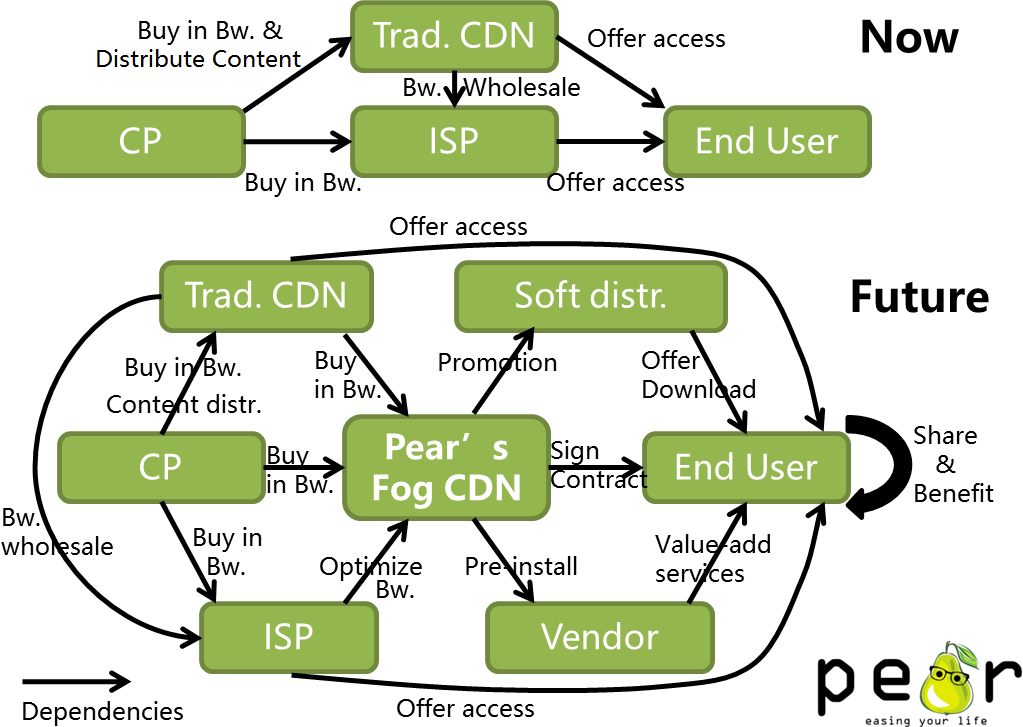
\includegraphics[width=.66\textwidth]{fig/biz/eco-system-change.png}
	\caption{Ecosystem change before and after Pear comes in.} \label{fig:eco-sys-change}
\end{figure}

The value proposition also illustrates the main reason why Pear is called ``Pear''. In ``The Three-Character Classic'' or ``San Zi Jing'', one of the most famous Chinese classic texts, an entire story is condensed into these twelve Chinese characters, means ``Aged four years, Rong proffered pears. Bear in mind, fraternally be kind''. The story mainly appreciates the then 4-year-old boy's virtue of being willing to share big pears to his elder and younger brothers. We extract the sharing spirit from this classic and find a better way to explain it with the success stories of Uber and Airbnb. Besides trying to make a profit, Pear is struggling to provide the best technical and economic means of P2P Internet sharing and to promote the concept of sharing resources for win-win situations via Fog Computing. 
\section{Services Offered}
Based on the concept and infrastructure of Fog Computing, Pear has the ambition of running hundreds of services that practise the philosophy of sharing economy. However, Pear is a company which surely needs revenue and profit in order to provide services consistently over time and grow to the next level. Thus, Pear is initially focusing on a few main services: 
\begin{enumerate}
	\item Fog CDN for Live Streaming and VoD (Video on Demand), aka Fog VDN;
	\item Fog Media Coding Service;
	\item Fog Storage Service;
	\item Fog VPN (Virtual Private Network);
	\item Fog Crawler/Spider;
	\item Fog BaaS (Blockchain as a Service);
	\item Fog Computing for IoT.
\end{enumerate}

\section{Revenue Streams}
Pear is a technology-driven start-up company, with limited financial resources. The primary revenue during the beginning years will be generated from a business-to-business (B2B) model. Pear is responsible for developing customised fog service platforms for business partners and will charge them appropriate prices that help them save costs and/or generate more revenue. 

Take Pear's Fog CDN service as an example: CPs currently obtain traditional CDN services, which are mainly charged according to peak bandwidth consumed and which typically range from HKD~$30,000$ to $100,000$/Gbps/Month. For Pear's Fog CDN service, the price charged will be within HKD~$10,000$ to $15,000$/Gbps/Month. Pear would invest part of the revenue into regularly scaling up the network infrastructure in order to build a stronger Fog CDN offering more bandwidth and better usability. 

\begin{figure}[ht]
	\centering
	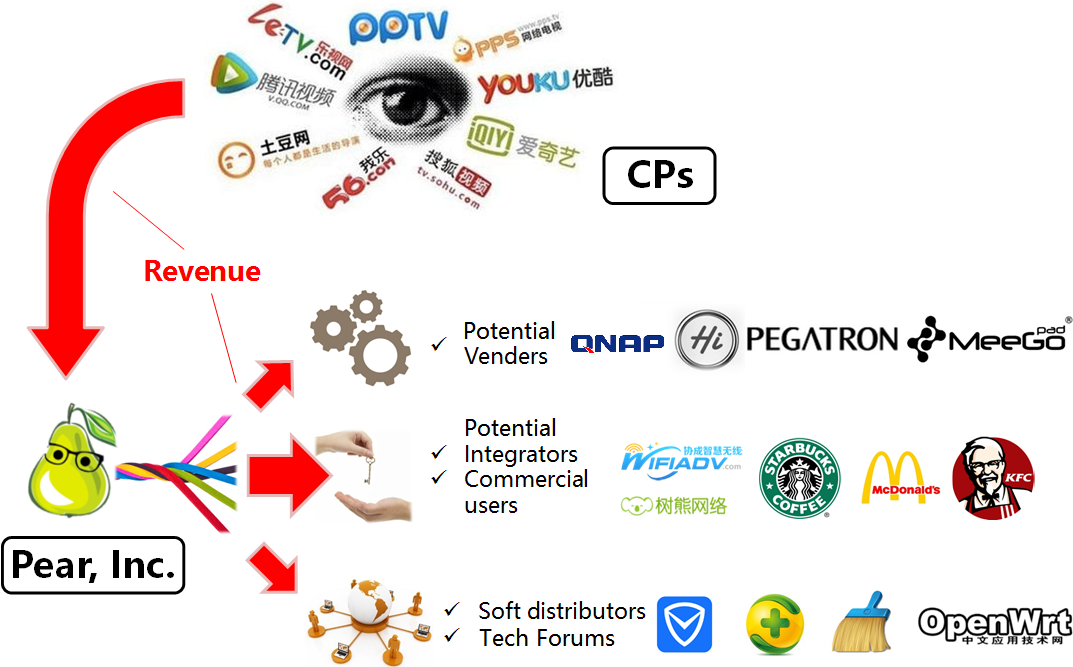
\includegraphics[width=.80\textwidth]{fig/biz/revenue_stream.png}
	\caption{Proposed revenue streams for Pear Fog's VDN service.} \label{fig:vdn-revenue-stream}
\end{figure}

\section{Distinctivenesses, Challenges and Risk Factors}
The brief introductions to Pear's technology and business have provided a rough picture of what Pear is, what it is doing and why it is doing it. Nevertheless, knowing how it works does not mean anyone can easily bring it into a real competitive market. Conversely, for projects like Pear's Fog VDN, the clearer people know about the details, the more likely they would realise that there is a solid barrier to success. 

The most difficult task throughout the development of Pear's Fog CDN platform has been to elegantly build the framework with pure C language. The platform interfaces with the front-end media control using HTML5 and JavaScript, with the back-end schedulers and servers using C++ and FastCGI, and with the embedded system programs using C and assembly. That is already beyond an ordinary full-stack engineer's range.

Howbeit, Pear can do even more. A traditional programmer would probably not be qualified to lead this project, because the Fog CDN platform also requires expert knowledge in streaming and network protocols, like WebRTC, HLS and MPEG-DASH, as well as various open P2P protocols. Even inside IT Giants, it is hard to find such guys with such versatile skills. Fortunately, Pear's three technology co-founders' backgrounds cover all these special criteria. Pear Fog is a demanding project in terms of hardware and software engineering, and it is also highly correlated to the newest Internet technology, which sets barriers for potential competitors. Only a special ops hardware and software team could try to do what Pear is doing.

In spite of all Pear's human capital, it does face some challenges and associated risks: 
\begin{enumerate}
	\item Pear does not yet have much capital investment. This shortage of funding could hinder Pear from scaling up rapidly. 
	\item Pear is overstretched with human capital. The team will have to work very hard and smart to achieve its goals in the given time frame.
	\item Pear still lacks its own market resources. It must initially solely rely on its partners, such as router vendors and CPs, and Pear knows it is a little bit over-reliant upon them. 
	\item The trial-test-and-pay nature of B2B businesses would make the revenue come relatively late. 
\end{enumerate}

Nevertheless, Pear's risk factors should also help Pear to work hard and work smart. We are young, eager and confident that Pear will grow much stronger soon. 
This is based on our working experience, input from experts and relationships in the CDN field and elsewhere that should encourage win-win cooperation.

\section{Product and Marketing Plan}
Among all the services we are offering, Fog CDN is Pear's featured product. It is a huge system, and we plan to steadily build it step by step, firmly. We believe the Fog CDN market will eventually capture people's attention. We also expect the Fog CDN to be the ever first successful product based on fog computing technologies. 

\subsection{Market Analysis}
Pear is an innovator in the CDN market. We are not able to tell whether our Fog CDN will completely replace the traditional CDN's role, but we aim to make it step gently into the traditional CDN market and gradually capture more and more market share until the two coexist and complement one another for a relatively long time in the future. 

\subsubsection{Target Customers}
In Pear's B2B Model, the targeted customers mainly refer to the CPs and traditional CDN service providers. 

Because of the inherent advantages of the background of one of the co-founders, Pear has a close relationship with the biggest video content provider in mainland China: Tencent Video. Pear's initial marketing efforts will focus on Mainland China since it is the largest market in the world and most of the co-founders are Chinese. 
Pear now is helping a new CDN provider to build a video cloud platform which implements part of Pear's Fog CDN technology aiming to help deliver the 4k video smoothly, and with a reasonable cost.

As user generated content (UGC) becomes more popular on the Internet, Pear expects to see some new types of CPs that leverage UGC business, such as BiliBili.com and ACfun.tv. Pear will also target them as customers in the first stage.

Due to the versatile Fog CDN infrastructure, as Pear grows, we can reuse this network to build the Fog VPN service with a high degree of usability. Pear plans to present consumers with the Fog VPN service in the second stage after the B2B business is proven to be viable.

\subsubsection{Market Characteristics and Trends}
From a commercial CDN market survey report, we can see that the Total Addressable Market (TAM) of the commercial CDN is increasing at a phenomenal rate, especially in China, see Figure~\ref{fig:CN-CDN-TAM}. 

\begin{figure}[ht]
	\centering
	\begin{center}
		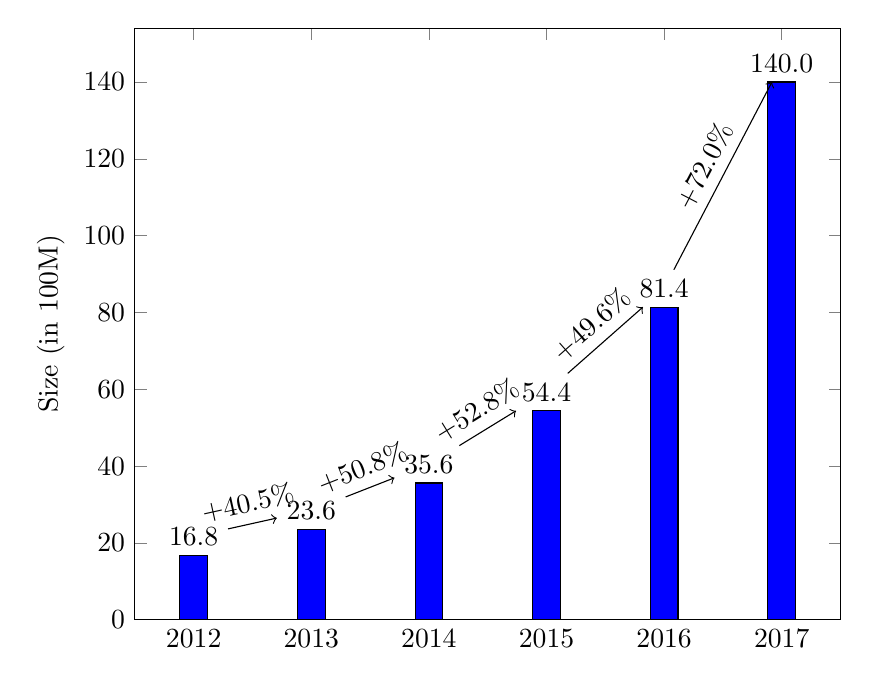
\begin{tikzpicture} %[>=latex]
		\begin{axis}[
		height=0.75\textwidth,
		symbolic x coords={2012, 2013, 2014, 2015, 2016, 2017},
		xtick=data,
		ymin=0,
		ylabel=Size (in 100M),
		enlarge x limits=0.1,
		%xticklabel style={text width=0.2\textwidth,align=flush left},
		]
		\addplot[ybar, axis on top, fill=blue] coordinates {
			(2012, 16.8)
			(2013, 23.6)
			(2014, 35.6)
			(2015, 54.4)
			(2016, 81.4)
			(2017, 140.0)		};
		\node (n2)[above] at (axis cs:  2012,  16.8) {$16.8$};
		\node (n3)[above] at (axis cs:  2013,  23.6) {$23.6$};
		\node (n4)[above] at (axis cs:  2014,  35.6) {$35.6$};
		\node (n5)[above] at (axis cs:  2015,  54.4) {$54.4$};
		\node (n6)[above] at (axis cs:  2016,  81.4) {$81.4$};
		\node (n7)[above] at (axis cs:  2017,  140.0) {$140.0$};
		\draw [->] (n2) -- (n3) node [midway, above, sloped] (tn1) {$+40.5\%$};
		\draw [->] (n3) -- (n4) node [midway, above, sloped] (tn2) {$+50.8\%$};
		\draw [->] (n4) -- (n5) node [midway, above, sloped] (tn3) {$+52.8\%$};
		\draw [->] (n5) -- (n6) node [midway, above, sloped] (tn4) {$+49.6\%$};
		\draw [->] (n6) -- (n7) node [midway, above, sloped] (tn5) {$+72.0\%$};
		\end{axis}
		\end{tikzpicture}
	\end{center}
	\caption{TMM of China Market.}\label{fig:CN-CDN-TAM}
\end{figure}

\begin{figure}[ht]
	\centering
	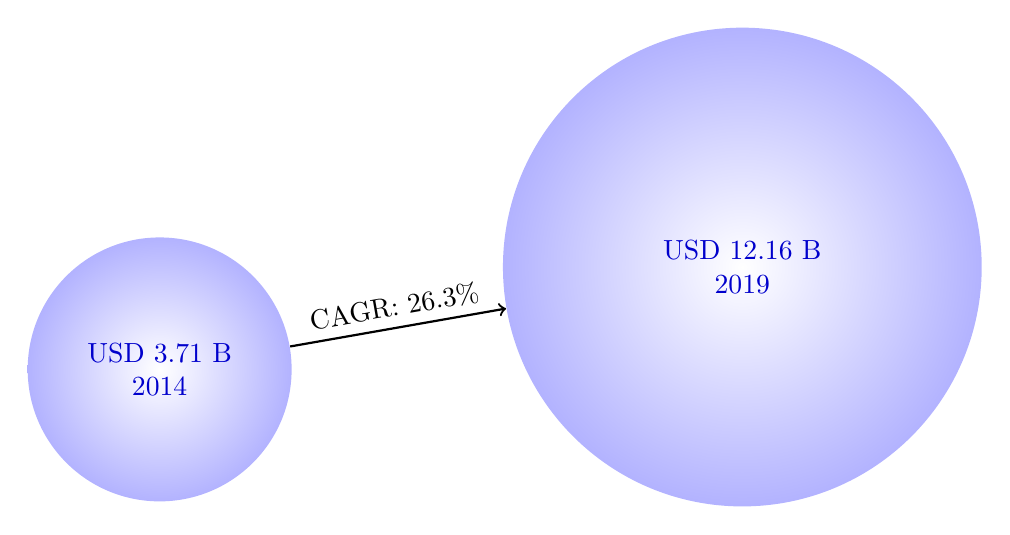
\begin{tikzpicture}
	\node(c1) [circle,shading=radial,outer color=blue!30,inner color=white,
	minimum width=1.855cm,align=center,text width=3cm] at (0.1,3.3) {\textcolor{blue!80!black}{USD 3.71 B\\ 2014}};
	\node(c2) [circle,shading=radial,outer color=blue!30,inner color=white,
	minimum width=6.08cm,align=center,text width=3cm] at (7.5,4.6) {\textcolor{blue!80!black}{USD 12.16 B\\ 2019}};
	\draw [->, thick] (c1) -- (c2) node [midway, above, sloped] (c1c2) {CAGR: $26.3\%$};;
	\end{tikzpicture}
	\caption{Cisco's world commercial CDN TAM growth expectations from 2014 to 2019.}\label{fig:World-CDN-TAM}
\end{figure}

According to a prediction by iResearch, the TAM of China's commercial CDN is expected to reach RMB 8.16 billion in 2016 with an annually increase at about 53\%. 
In fact, we have witnessed that all previous CDN market size predictions were eventually proven to be far behind the real growth. For example, in a Cisco white paper published in 2014, the world's commercial CDN TAM in 2012 was predicted to reach USD 12.16 billion at a CAGR of 26.3\% as depicted in Figure~\ref{fig:World-CDN-TAM}, while a report\footnote{\url{http://www.researchandmarkets.com/research/8vnkvv/mobile_cdn_market}} issued in 2015 suggested that the mobile CDN market alone will grow from USD 2.11 billion in 2015 to USD 13.40 billion by 2020, at a CAGR of 44.7\%. 

The fact is telling us: data traffic demand tends to run far over the commercial CDN capacity. Moreover, the gap between demand and supply is becoming wider and wider. When we compare China's market and the World's, we find that commercial CDN only serves 8-10\% of total Internet data traffic in China, while in the US, commercial CDN has already been serving around 50\% Internet data traffic. This is another reason why Pear is focusing on the China market in the first stage.

Apart from that, we expect that the demand for commercial CDN will last for long, so we are sufficiently confident with its market, even in the global depression. This is because commercial CDN mainly serves online video, games and related entertainment industries that are expected to perform very well regardless of the economic outlook. History shows that Broadway and Hollywood thrived during the Great Depression, so unless there is a war or global cataclysm, we expect similar favourable conditions in the CDN market. 

\subsubsection{Revenue Potential}\label{revenue-potential}
During stage one, we have a simple method to estimate the revenue of this business:
Assume a CP needs 8Tbps bandwidth for delivering its video content, 1\% of its traffic is 80Gbps. For the general case of CDN bandwidth price, HKD~$30,000$/Gbps/Month, 1\% of his traffic will cost HKD~$2.4$ million. For our Fog CDN, we need only around $8,000$ signed smart routers to share their idle uploading peak bandwidth less than 10Mbps. With our pricing strategy, we will only charge this CP HKD~$1.2$ million as the service price. In this case, the CP will save HKD~$1.2$ million to and be able to purchase the broadcasting rights of more video content, and we will also have the flexibility to manage our income. For example, we could return HKD~$600$k cash or equivalent VIP memberships to the $8,000$ signed users, and retain left HKD~$600$k as profit.

The above scenario only shows the starting case of taking 1\% of this CP's data traffic. The business is clearly scalable, because if we have more signed home/business routers and idle bandwidth, we will be able to take more traffic volume. Above all, there is only one CP for this illustrative example. In reality, we can provide this Fog CDN to multiple CPs with both a sweet price and good quality. Our target is to serve as many CPs as possible within our capability. 

\subsection{Product \& Service Plan}
Pear has divided its product and service marketing plan into three stages, as describes in Table~\ref{tb:product-market-plan}. 
\begin{table}[htb]
	\centering
	\caption{Pear's first three stages of its product and service and marketing plan.}\label{tb:product-market-plan}
	\footnotesize
	\begin{tabular}{p{0.11\linewidth}p{0.28\linewidth}p{0.28\linewidth}p{0.28\linewidth}}  
		\toprule
		Stage &    Stage 1    & Stage 2 & Stage 3 \\
		\midrule 
		Time & Year 0-1.5 & Year 1.5-2 & Year 2+ \\
		End-users & Low awareness of Pear's Fog Computing \& sharing economy philosophy & High awareness of Pear's services & Actively install Pear to their own devices to join Pear's world\\
		Cooperating Firms & {Pear has no user base at this stage. We need to cooperate with large user-base companies to build up the Pear Virtual Network: HW: MeegoPad, AllWinner, Huawei, Intel; CP: Tencent Video, imeme.tv; Pear's own device: in design} & {Pear will have built up a broad-range network. Cooperating firms (mostly CPs) gradually become Pear's customers} & {Pear will not be depending solely on the end-user base of cooperating companies}\\
		Target Customers & {Testing with cooperated firms; small or medium CPs} & {Large CPs, especially cooperating companies} &    All web CPs\\    
		\bottomrule
	\end{tabular}
\end{table}

\subsubsection{R\&D Milestones}
Pear plans to launch the Fog email delivery and Fog CDN services at the same time since quite a number of elements overlap. It is highly efficient to reuse the resources while achieving multiple targets, although the email delivery source may not be used as thoroughly as the Fog CDN. The detailed milestones are shown in Table~\ref{tb:rd_milestone}. 
\begin{table}
	\centering
	\caption{Pear's R\&D Milestones}\label{tb:rd_milestone}
	\small
	\begin{tabular}[t]{ccp{0.68\linewidth}}  
		\toprule
		\multicolumn{2}{c}{Period} \\
		\cmidrule(r){1-2}
		From & To & {\textsc{~~~~~~~~~~}Description}\\
		\midrule
		01/02/2016 & 01/03/2016  & {1. Basically finish the protocol, API, and architecture designs for Pear's fog computing system.\newline 2. Establish one or two partnerships in which we help partners solve cost optimisation problems and hopefully gain some referrals and/or more attractive contracts.}\\
		01/03/2016 & 01/09/2016    & {Implement Pear's fog computing protocols on the firmware of Pear's routers and/or IPTV set-top boxes (all-in-one devices).}\\
		01/09/2016 & 01/10/2016 & {1. Enable Pear's fog computing system on the live streaming platform(s) of partner(s) of Pear.\newline 2. Provide open source versions of some components of Pear's fog computing project under MIT, Apache, BSD or GPL license(s), and at the same time maintain a commercial version.\newline 3. Create real impacts in the corresponding industry, especially the open source communities.}\\
		01/10/2016 & 01/02/2017 & {1. Complete the project developed for Partner 1 (Probably ``Fog'' email delivery and HD video transmission).\newline 2. Complete the project developed for Partner 2 (``Fog'' live streaming service platform).}\\
		01/02/2017 & 01/12/2017    & {Launch and complete the project developed for Partner 3 (“Fog” Multimedia CDN)}\\
		\bottomrule
	\end{tabular}
\end{table}

\subsection{Marketing and Sales Strategy}
We have carefully thought through the four Ps of marketing: product, promotion, place, and pricing. Our strategies for each of these are introduced below. 

\subsubsection{Product Strategy}
Pear's Fog CDN service is designed to run like a duet: it serves both the CPs \& ISPs and the end-users simultaneously, like a precise driving gear powering its driven counterparts automatically.

Pear is already prepared to cooperate with ISPs who have a large user base but are weak in cloud data centres (such as China Mobile) and hardware vendors (such as Huawei). Through this fundamental work, the end-users will enjoy:
\begin{enumerate}
	\item Faster Internet access and a better video streaming experience;
	\item Remote control, monitoring and management for the signed smart devices;
	\item Real cash/coupons or VIP service as a reward for sharing their idle bandwidth.
\end{enumerate}

Pear is ready to provide high-quality CDN services, initially mainly for online video CPs, promising to reduce operating costs significantly. For these wise content providers, they can enjoy: 
\begin{enumerate}
	\item Better streaming quality and transmission efficiency of CDN services;
	\item Better geographical access coverage;
	\item Significantly lower content delivery cost;
	\item ``Flash-crowd'' and ``bottle-neck'' headaches minimisation.    
\end{enumerate}

\subsubsection{Promotion Strategy}
Pear plans to use common channels, like social media and mass media, for public awareness.
At the same time, Pear is leveraging media resources of device vendors (agreed), Intel (agreed), Tencent, and JD.com crowd-funding for promoting the fog computing devices and services. There are three main methods Pear is going to use for promotion in B2C model as illustrated in Figure~\ref{fig:promotion-strategy}.  
\begin{figure}[ht]
	\centering
	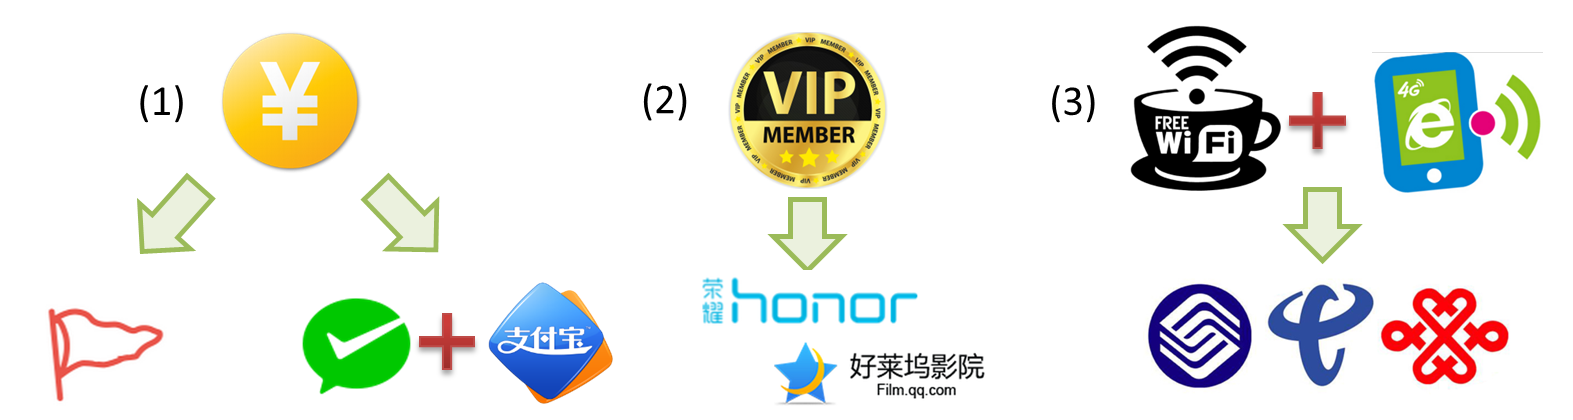
\includegraphics[width=.80\textwidth]{fig/biz/promotion_strategy.png}
	\caption{Promotion strategies for Pear's B2C Model.} \label{fig:promotion-strategy}
\end{figure}
\begin{enumerate}
	\item Cash rewards or interest-free instalments as incentives. Pear even can deliver the smart routers for free to end-users who sign an agreement to stay online 24/7 to provide bandwidth for the Pear Fog, thus helping the network accommodate more traffic or content delivery volume.
	\item CP VIP memberships to leverage activities or direct exchange with end-users, so they will contribute bandwidth to support more network traffic.
	\item Cooperation with the ISPs and/or telecom operators, such as China Mobile. Pear will be able to provide them with the scaled end-users' contributed traffic volume through cellular phones' data networks.
\end{enumerate}

\subsubsection{Place and Channel Strategy}
Initially, Pear must partner with vendor companies to bundle Fog services with their smart devices, such as routers and TV boxes, as well as mini PCs to establish a wider user base among the general public.

For most of the initial stage, Pear will not face consumers directly, so Pear must focus on its B2B channel to first help vendors with their bandwidth needs. However, at a later stage, Pear would pay much more attention to its B2C channel, which is related to the life and death of Pear in the long run. Otherwise, vendors would eventually develop their own in-house fog platforms and go around us, thus leaving us without work to do. 

Facing customers will not only help with our longevity, but it will also help us better understand their needs and wants and serve them directly. Thus, Pear will pay full attention to all possible channels that could reach the consumers.
% Only when we could face with customers directly, we have the initiative of development and going concern. So Pear would pay full attention to all possible channels that could reach the consumers.

\subsubsection{Pricing Strategy}
For Pear's Fog CDN service, its price will initially be about HKD~$12,000-15,000$/Gbps/month. This price is about 40\% of the currently cheapest traditional CDN competitors in Mainland China. Pear is also considering other flexible pricing schemes for different scenarios, {\em e.g.}, by total traffic/size of data, by user base, by coverage of outlying regions and edge ISPs, and by the load shifting effect. Pear's aim is to always be to provide equivalent or better quality CDN services at less than half of the original pure-traditional CDN price. 

\subsection{Competition}
Pear is an innovator in the relatively mature traditional CDN market. We will face challenges from existing giants who are also considering Fog CDN as well as from the other innovators with similar Fog CDN services. On the other hand, these competitors could also be Pear's customers and partners. Thus, Pear keeps an open mind to the competition and expects all interested communities and individuals to join in the fog computing world to explore and contribute. One proof of this open-mindedness is that Pear has already kept and will always keep all wheel-like core components open source. This is similar to the early Microsoft model of allowing its software (MS-DOS) to be freely copied all over the world, which gave it a clear victory over IBM's PC-DOS, which became the standard for most PCs in the 1980s. IBM did not foresee the rampant of ``file sharing'' of PC retailers in countries outside the US, nor did it expect Bill Gate's tiny start-up to actually gain so much from it. This was all thanks to a non-exclusive agreement that the tiny start-up signed with the computing giant in 1980 \cite{ms-ibm-dos}. 

\subsubsection{Traditional CDN Competitors in Mainland China}
In China, there are two outstanding traditional CDN giants to whom Pear is paying attention: ChinaNetCenter and ChinaCache.

In 2014, ChinaNetCenter had a market share of about 43\%, and ChinaCache about 37\%. In 2015, ChinaNetCenter had revenue over RMB 2 billion, with a market capitalization at around RMB 30 billion, and ChinaCache had a market capitalization at USD 185 million while its revenue was around USD 220 million. 

Among the two CDN giants, ChinaCache is more willing to access new technology, since it has recently signed a cooperation contract with HiWiFi Router and Youku LuYouBao. Pear looks upon ChinaCache as one of the biggest competitors, and sincerely admires its strategy as well as executive power. On the contrary, Pear looks forward to potential cooperation opportunities with ChinaNetCenter. 

\subsubsection{New-born Competitors in China Mainland}
From 2015 till now, Pear only has two new competitors in the Fog CDN market: Xunlei (Thunder) XYCDN\footnote{\url{http://www.xycdn.com/}} and Youku LuYouBao\footnote{\url{http://yj.youku.com/luyou}}.

Xunlei originally is a download manager and Peer-to-peer software developed by Thunder Networking Technologies, supporting HTTP, FTP, eDonkey, and BitTorrent protocols. As of 2010, it was the most commonly used BitTorrent client in the world. On 24 June 2014, it went public on the Nasdaq Stock Exchange, raising 88 million USD. Xunlei's advantage concentrates on file downloading techniques which are essential for Fog CDN. Moreover, now Xunlei has just adjusted their strategic direction to ``crowd-sourced CDN''. Their CDN, called XYCDN, is their featured product right now. The product is still naive but has efficient iterations. Xunlei has just announced their 2nd Generation ZhuanQianBao miner: a low-cost mini server which when plugged into users' home routers, is ready for sharing not only idle bandwidth but also storage.

Youku Tudou Inc. is one of China's biggest video CPs, having a market capitalization of over USD 5 billion. It is aggressively investing in innovative technology that enhances its services while reduces its cost. Recently, it was reported that Youku had sold over 500k 1st generation LuYouBao intelligent network terminals in 2015. Different from the Xunlei ZhuanQianBao miner, LuYouBao is a smart router with full functions. Youku LuYouBao signed a co-development contract with ChinaCache in 2015, so Pear sees these joined forces as great competitors. 

\subsubsection{New-born Competitors outside of the Greater China}
Unlike the Chinese competitors who focus on CDN hardware, Pear's international competitors are leading the software and platform design for the P2P CDN industry.

One of the competitors is named Peer5. Established in 2012, Peer5 is a CDN provider that leverages WebRTC (see Appendix B) to improve content delivery with the assistance of P2P technologies. Peer5's offerings include a live streaming CDN, a radio streaming CDN, a big object downloader, a VoD CDN and image loading service. Peer5 has already received angel investment and has over ten staff working full-time. The idea of leveraging WebRTC protocol coincides with Pear's Fog CDN R\&D plan. This fact gives Pear confidence, and Pear appreciates Peer5's courage to be the first mover to help the P2P CDN industry get a second wind. Currently, Peer5 is not doing much in China, but if Pear expands outsides of China, especially in western countries, Peer5 is likely to be a competitor.

\subsubsection{Pear's Comparative Advantages}
\begin{itemize}
	\item Pear's comparative advantages over traditional competitors\\
	Although a traditional CDN is easy to schedule in the initial stage, two critical shortcomings lie in front of a traditional CDN company when it is going to scale up. One is the cost. Even for the biggest traditional CDN provider with sophisticated cost control, the bandwidth's price is still two to three times as much as that of the Pear's Fog CDN. The other is the geographic limitation. Since traditional CDN deployment requires data centres, the outlying regions and edge ISPs typically meet trouble to set up CDN servers.
	
	On the contrary, because end-users' smart devices are working as distributed CDN servers, Pear's Fog CDN servers can instantly work anywhere Internet users exist. Pear will never face the same problems as its traditional CDN competitors do when scaling up or expanding geographically. This is similar to the advantage Microsoft had over  IBM in the 1980s. 
	
	\item Pear's comparative advantages over new-born competitors in China\\
	The new-born Chinese competitors all have one problem in common: neglecting the system architecture design at the beginning. It is understandable that companies have pressure to bring in income as soon as possible. However, in Xunlei XYCDN's case, stuffing the miner with outdated HTTP server techniques along with proprietary protocols as a crowd-sourced CDN server, has created hidden risks in case other competitors prove that the WebRTC protocol is overwhelmingly useful for Fog services, on which Pear is now working. With old and proprietary (and exclusive) protocols and modules, Xunlei's CDN service is completely Web-unfriendly: the end-users need to install apps or clients; the served CPs need to modify their source code to call Xunlei's services as well. Thus, they are not user and CP transparent. So these issues will be a stumbling block to Xunlei in the future if they cannot realise it and rectify it in time. 
	
	The differences between Xunlei's hardware and Pear's hardware are briefly summarised in Figure~\ref{fig:hw-comp-xunlei}.
	\begin{figure}[ht]
		\centering
		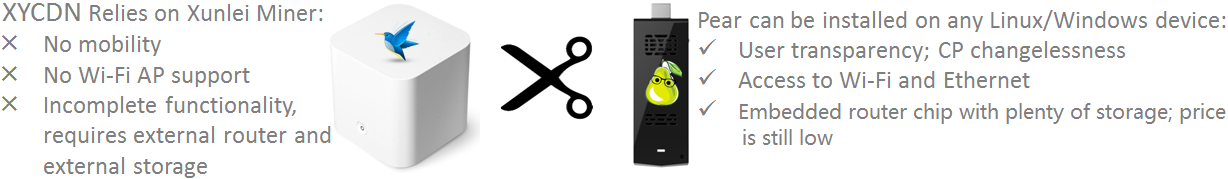
\includegraphics[width=.88\textwidth]{fig/biz/hw_comp_xunlei.png}
		\caption{Comparison between Xunlei's and Pear's hardware.} \label{fig:hw-comp-xunlei}
	\end{figure}
	
	\item Pear's comparative advantages over new-born global competitors\\
	When we consider competitors like Peer5, it is rather respectful and admirable to have such a strong R\&D team fighting on the frontier. WebRTC is an advanced, future-oriented protocol for communication between any browsers. It can easily enable P2P communication and maintain the web-friendliness at the same time. That is why Pear shares a similar concept for implementing WebRTC protocol as the infrastructure of Pear's Fog CDN. 
	
	However, there is one problem that Peer5 may have considered but has no solutions for right now. Peer5's CDN service is based on the web browsers on desktop PCs, whose behaviour is unpredictable because the user behaviour behind them is random. In large-scale commercialised services, Peer5's performance will be affected, and they need to find a way to try to keep most of the nodes always working online. Bur it is hard, because they have no enough monetary incentive to encourage the end-users to keep their PCs and browsers running 24/7.
	
	Pear has chosen another approach --- a deliberate method to ensure each nodes' stability as a Fog CDN server. We are embedding the WebRTC protocol directly into routers with pure C language.
	Experienced engineers will know the difficulties on the way to success, and we are determined to achieve success on the way. We are now working to overcome the highest hurdles for popularising the Fog computing technology into reality. We are also seeking talented engineers and professionals to join us. 
	
	Pear has another inherent advantage: geographic proximity. Pear is based in Hong Kong and Shenzhen, which enables us to develop connections with various router, TV-box and mini PC vendors in these two thriving cities. This makes it easy to cooperate and receive technical support more easily, compared with Peer5 or other competitors outside China.
	
	\item Pear's comparative advantages over other start-ups by fresh graduates\\
	Pear's founders have an unusual background. The three of them combined have a dozen years of professional experience in the networking field, and two of them are currently pursuing postgraduate degrees at HKUST in the prestigious TLE program. Combining their connections and resources from the industry with their advanced research work, they have put together a dream team for Fog CDN services and smart router innovation. They are not merely IT guys. 
	
	With technical experience, not are they academics with lots of conceptual knowledge but no practical industry experience. They have the best of both worlds.
	%Pear is a little bit unusual for its background. Three of the co-founders have years of working experience, and two of them are back to university although they already have achievements in their career. They brought back the connections and resources from the industry and through the research work in HKUST, they polished their entrepreneurship ideas. Finally, with endless passions, these guys started the new story at the ever highest point, and this is how pear begins.
	
	%Moreover, also this is the one difference between Pear and the other start-ups mainly composed of PhDs and professors who have never or rarely been deeply involved in the real industry. 
\end{itemize}
In summary, Table~\ref{tb:features-pearcompetitors}, Figure~\ref{fig:cost-performance-competitors} and Figure~\ref{fig:all-essences-advantage} provide comparisons of Pear with its primary competitors. 

\begin{table}[hb]
	\footnotesize
	\centering
	\caption{Features of Pear Fog VDN and its competitors}\label{tb:features-pearcompetitors}
	\begin{tabular}[t]{p{0.08\linewidth}p{0.05\linewidth}p{0.05\linewidth}p{0.06\linewidth}p{0.05\linewidth}p{0.25\linewidth}p{0.14\linewidth}p{0.10\linewidth}}  
		\toprule
		Product & Wi-Fi AP & Media CDN & Patented & Rebate profit to end-users & Price @ CP side & Coverage & Targeted Customer\\
		\midrule
		Pear & Yes & Yes & Yes & Yes & HKD~$12$K/Gbps/month & Worldwide\tablefootnote{We start with the Greater China and branch out in Asia; One Belt, One Road (OBOR) countries will also be target regions: they have 60\% of the world's population and way be happier with fog.} & Any CP\\
		Thunder XYCDN & No & Yes & No & Yes & CNY~$10$K/Gbps/month & China & Large CP\\
		ChinaNet-Center & No & Yes & No & No & CNY~$60$K+/Gbps/month    & Mainly China & Traditional Websites\\
		Akamai & No & Yes & Yes & No & Depends on service region,  generally expensive & Worldwide (except China) & Traditional Websites\\        
		\bottomrule
	\end{tabular}
\end{table}

\begin{figure}[ht]
	\centering
	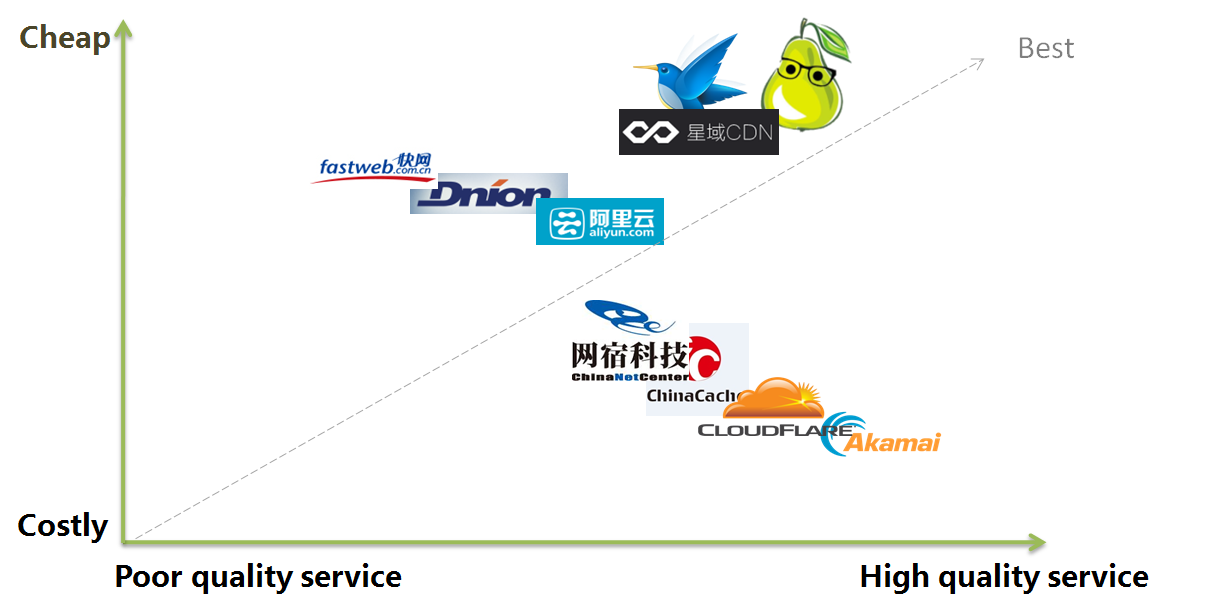
\includegraphics[width=.8\textwidth]{fig/biz/cost-performance-competitors.png}
	\caption{Cost/Performance view on Pear and its competitors.} \label{fig:cost-performance-competitors}
\end{figure}

\begin{figure}[htb]
	\centering
	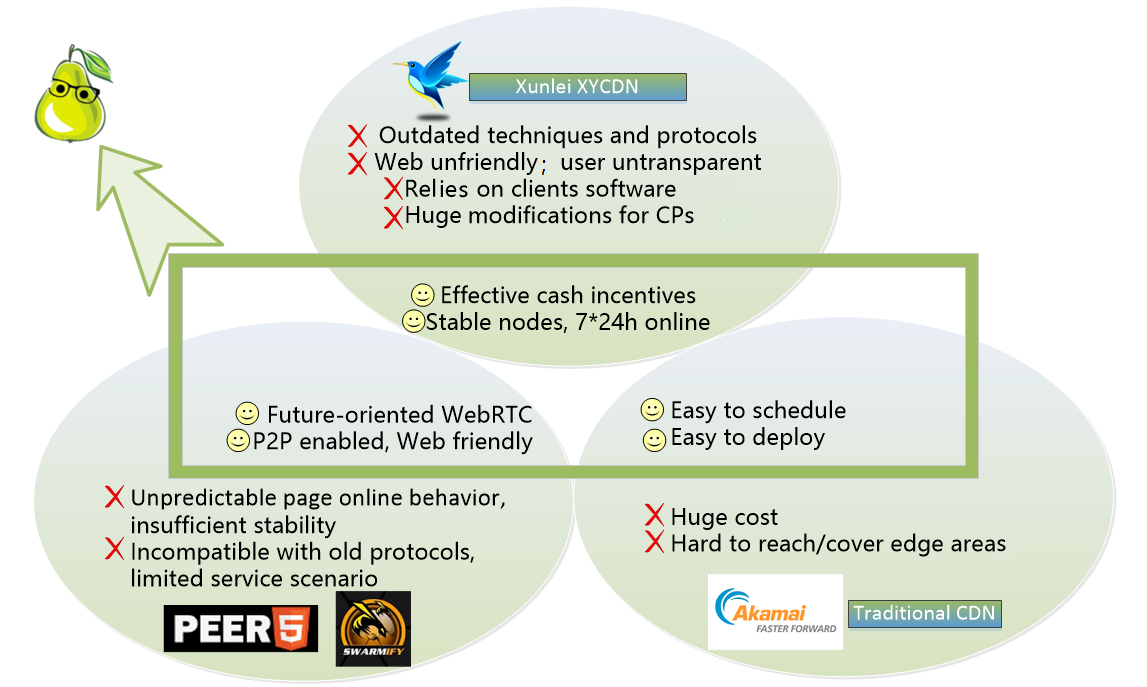
\includegraphics[width=.8\textwidth]{fig/biz/all-essences-advantage.png}
	\caption{Illustration of why Pear is ``tasty''.} \label{fig:all-essences-advantage}
\end{figure}

\subsubsection{Potential Competitors in Emerging Fields}
Potential competitors in emerging fields may be grouped into two categories: 
\begin{itemize}
	\item Cloud WebRTC Service Providers 
	\item IoT Fog Computing Service Providers
\end{itemize} 

The first group is characterised by products which are enabling mobile apps and web pages with real-time communication capabilities. They offer the web and mobile SDKs that connect to their cloud WebRTC services and charge business users based on total connections, sessions or bits. An example is Agora, founded by YY Live's co-founder and ex-CTO. Agora raised USD 25.9 million in its Series A and B investments in 2015. It then sponsored the world's most influential WebRTC conference and translated a WebRTC standard book to Chinese, which made it the most well-known WebRTC-specialised technology company in China. 

The second category is characterised by businesses that are bringing intelligence to the edge. FogHorn is a such example. It provides an edge software stack for industrial IoT that ingests the data from sensors and industrial devices onto a high-speed data bus and then executes user-defined analytics expressions on the data stream to gain insights and optimise the devices. ForHorn secured USD 12 million in Series A funding on 27 July 2016. 

Pear acknowledges strong competition from these competitors. However, viewed from another angle, the competition will help bring the WebRTC and Fog concepts to the industry. Pear's initial revenue source is expected to be from services to Cloud providers, while its own emphasis is the Fog. The Fog requires wide coverage by a huge amount of enabled nodes, while the Cloud only requires a simple ``one-click-enabling''. 

\subsection{Strategic Partners}
Before introducing Pear's strategic partners, it is necessary to have a full view of China's “CP+Vendor+CDN” ecosystem in Figure~\ref{fig:cp-vendor-cdn}.
\begin{figure}[ht]
	\centering
	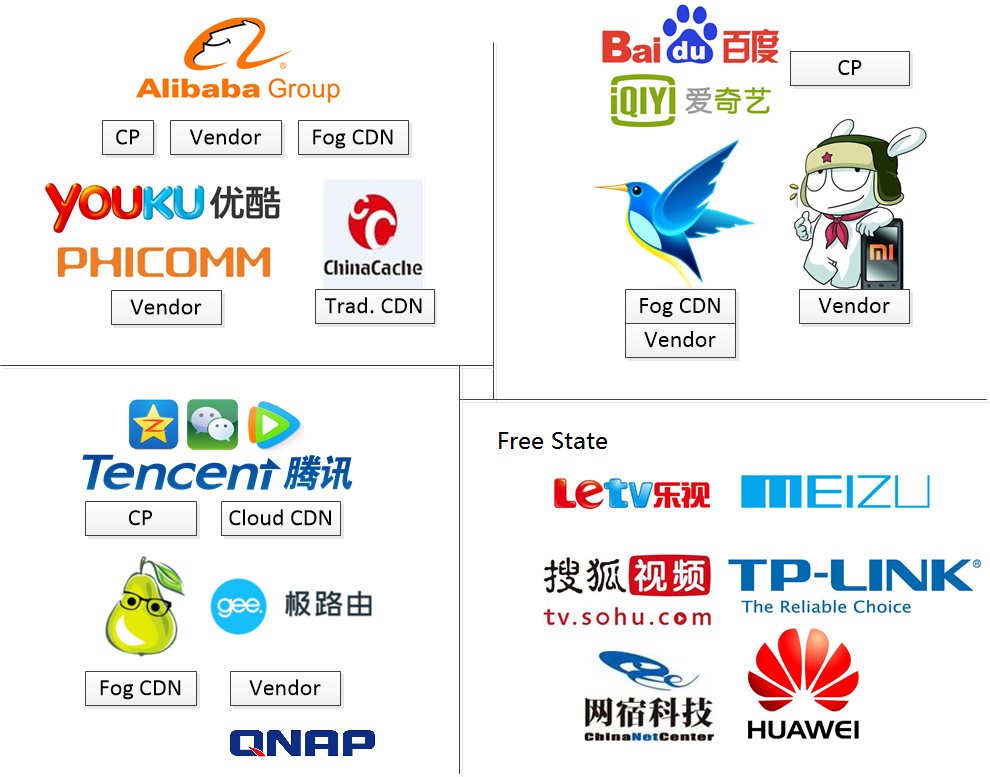
\includegraphics[width=.75\textwidth]{fig/biz/cp-vendor-cdn.png}
	\caption{Rough view of power distribution in the ``CP+Vendor+CDN'' ecosystem.} \label{fig:cp-vendor-cdn}
\end{figure}

It is not surprising to see the ``BAT (Baidu-Alibaba-Tencent)'' allied pattern in the current market; after all, they are the only three dominant giants in China's IT industry. Right now, Pear has cooperation with Tencent. In the meantime, Pear is trying to be neutral to all CPs, since the quickest way to promote the Fog CDN service is to open it to everyone.

We can see that there still exist neutral or unallied formidable players in the industry, and Pear is aiming at prioritising cooperation with these participants, such as Huawei, Pear has already negotiated with Huawei and has reached an initial agreement on co-developing the APIs on top of Huawei Honour router's customised firmware. 

\subsubsection{Vendor Partners}
Pear Fog CDN edge programs are fundamentally designed to be cross-platform and can be installed on every smart device with Windows or Linux OS, {\em e.g.} home routers, TV boxes, PCs, self-hosted servers and even cellular phones. To achieve the optimal result, we chose routers as the best candidates mainly because:
\begin{enumerate}
	\item they can ensure a high probability of 24/7 online connectivity;
	\item they have a good chance of obtaining public IP addresses, which reduces of at least one layer of NAT traversal, which can mean much better accessibility. 
\end{enumerate}

Pear will not have hardware manufacturing capabilities until January 2017, so Pear has acquired several hardware partners for developing and testing Pear's Fog CDN services.

\begin{itemize}
	\item NetGear Hong Kong\\
	NetGear is a US-headquartered global networking company that specialised in producing high-end routers for retail and business markets. NetGear Hong Kong has offered Pear and RADICA four Nighthawk R8000 and one R7000 routers (see Figure~\ref{fig:netgear-r7000-r8000}) for developing and testing the Fog email delivery project. RADICA also proposed to deliver a few thousands of routers in Hong Kong and Taiwan to launch a fog computing platform. 
	\begin{figure}[ht]
		\centering
		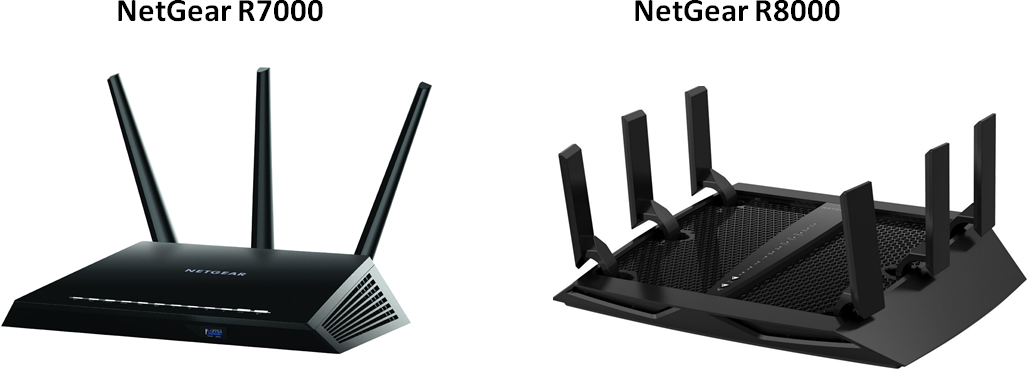
\includegraphics[width=.7\textwidth]{fig/biz/netgear-r7000-r8000.png}
		\caption{NetGear Nighthawk R7000 and R8000 Wi-Fi Routers.} \label{fig:netgear-r7000-r8000}
	\end{figure}
	\item Huawei Honor\\
	Huawei Honor has independent R\&D and marketing teams. In 2015, they sold over two million ``Honor Routers''. The Huawei Honor R\&D team has agreed to open their proprietary APIs to Pear to enable Pear's fog computing services. However, after some small trials, Pear engineers found Honor's VM environment is currently not friendly to native C program development. The porting work has been put on hold for one year. 
	\item QNAP\\
	Headquartered in Taiwan, QNAP is the 2nd largest global NAS vendor. Intrigued by Pear's Sharing Fog Computing concepts, QNAP had a meeting with Pear in Shenzhen in early autumn 2016. QNAP expects to see when Pear schedules the computational resources of 5,000,000+ QNAP devices (see example types in Figure~\ref{fig:qnap-x51}) worldwide and brings value added to the device owners. QNAP is willing to promote Pear's software with its own channels. After that meeting, QNAP offered Pear the latest SDK (called QDK) to make the development easier. A tentative plan is to beta test the software by January 2017 and launch the service by March 2017.
	\begin{figure}[ht]
		\centering
		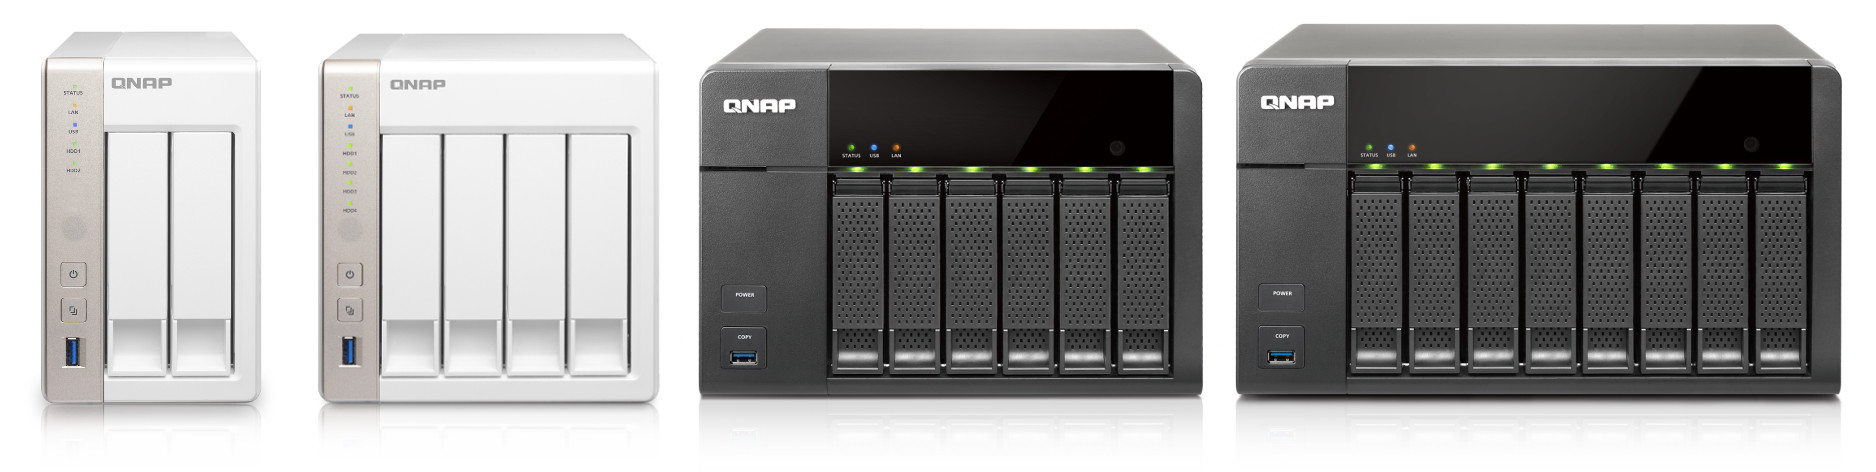
\includegraphics[width=.7\textwidth]{fig/biz/QNAP_x51.jpg}
		\caption{QNAP x51 Series.} \label{fig:qnap-x51}
	\end{figure}
	\item MeegoPad\\
	MeeGoPad was the earliest vendors to offer its hardware for Pear's R\&D and testing. In fact, MeeGoPad is the biggest ODM \& OEM for Intel Compute Stick product line in China. They have promised to develop a customised carrier to run Pear's fog services. Pear is preparing the supporting software for the so-called \emph{Pear Stick} or \emph{Pear Sharing Box} at this moment. Beta testing is scheduled for January to March 2016, and Pear hopes to begin marketing it in April 2017 and shipping it to vendors and crowd-funding platforms in May 2017.
	\begin{figure}[ht]
		\centering
		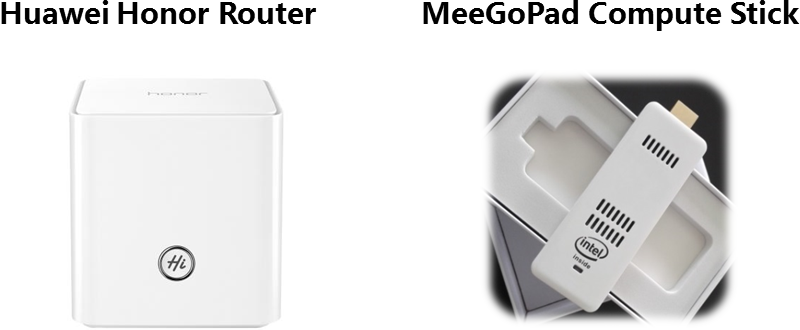
\includegraphics[width=.7\textwidth]{fig/biz/huawei-honor-and-meego-stick.png}
		\caption{Other carriers of Pear Fog: Huawei Honor Router and MeeGopad Compute Stick.} \label{fig:huawei-honor-and-meego-stick}
	\end{figure}
\end{itemize}

\subsubsection{CDN Partners}
Shanghai Maichuang Network Technology Co., Ltd. (aka Tan14\footnote{\url{https://www.tan14.cn/}}) is a CDN start-up company with seemingly strong financial strength and based in Shanghai. They have admirably extensive connections with CPs, and their customers have already generated enough profit for scaling up and investing in R\&D. Currently, they have more than 80 CDN nodes distributed in Mainland China and Hong Kong as well as Taiwan.

Pear and Tan14 have reached a cooperation agreement to build an entirely new cloud \& fog integrated platform for live streaming by the end of 2016. Pear is responsible for architecture design and software implementation coordination, while Tan14 has promised the customers and the investment. Hopefully it will be a win-win partnership.

\subsubsection{CP \& SP Partners}

\begin{itemize}
	\item Tencent\\
	Tencent Video is one of the biggest online video content providers in Mainland China. It has a private CDN to support the growing bandwidth demands. However, as Figure~\ref{fig:tencent-youku-cost-growth} depicts, it is now facing a serious cost/revenue bottleneck. Tencent Video and Pear have also reached an agreement for scheduling and testing the Pear Fog CDN when Pear's active routers arrive at a certain number. As mentioned in Section~\ref{revenue-potential}, Tencent Video will immediately resolve their cost bottleneck once they are equipped with Pear's Fog CDN.
	Besides Tencent Video, Pear also has oral agreements with two other Tencent subsidiaries Qzone's and QQ Video Album's teams plan to schedule the video content delivery through Pear's Fog CDN when it is ready.
	\begin{figure}[ht]
		\centering
		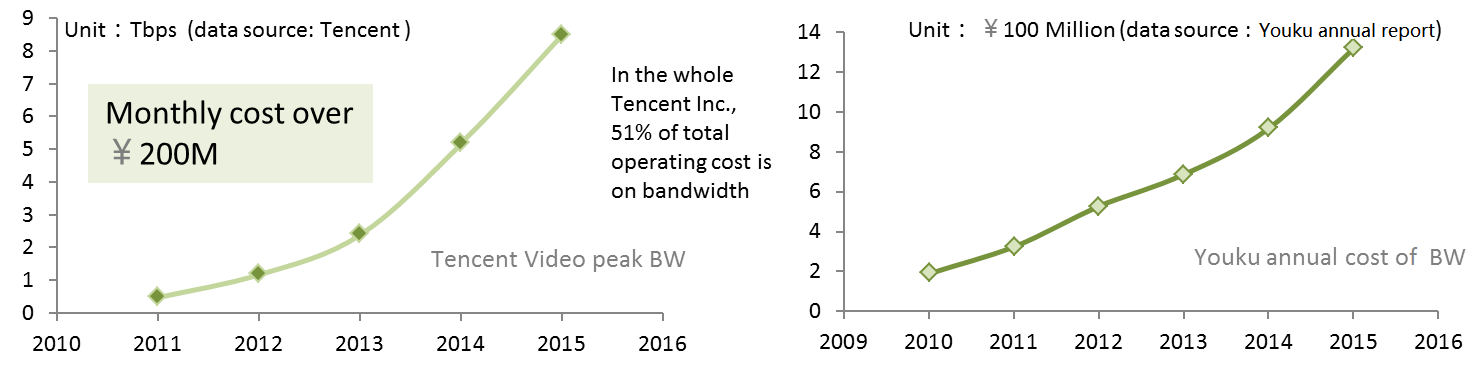
\includegraphics[width=1.00\textwidth]{fig/biz/tencent-youku-cost-growth.png}
		\caption{Some CPs' cost growth rate.} \label{fig:tencent-youku-cost-growth}
	\end{figure}
	
	To summarise the partnership with Tencent: Pear has the chance to test the Fog CDN serving:
	\begin{enumerate}
		\item the largest online video platform in China (in terms of traffic); 
		\item the largest social networking service in China;
		\item and one of the largest photo album platforms in the world.
	\end{enumerate}
	
	\item RADICA\\
	RADICA Systems is an HKUST alumni-owned IT company based in Hong Kong. With 15 years of experience, RADICA has mainly helped Asia Pacific brands and enterprises to effectively perform direct marketing. Over 300 enterprises are now their customers. With the aid of Pear's fog computing platform, RADICA expects to be able to provide its current services at an astonishingly lower price so that they can hopefully increase their customer base.
	
	RADICA, Pear and NetGear are now jointly launching a ``fog email delivery'' project. Pear is responsible for the software and RADICA is responsible for the customers and technology support for the email servers'resources. Currently, the project is successful in the first stage; the prototype is working online. In the second stage after Autumn 2016, RADICA and Pear will start a large-scale test in a real commercial scenario. This fog email pushing project is critically important to Pear since it contributes to building the fundamental framework of Pear's fog computing network. Pear will save time in developing its Fog CDN and Fog VPN infrastructures thanks to this fog email pushing product. 
\end{itemize}

\subsection{Operating Plan}
\subsubsection{Hiring and Development Plan}
Pear plans to scale up to around 10-15 staff by mid-2017, including three owners. Details are in Table~\ref{tb:hiring-plan}. 
\begin{table}[ht]
	\centering
	\caption{Pear's Hiring Plan.}\label{tb:hiring-plan}
	\begin{tabular}[t]{llr}  
		\toprule
		Time (mm/yyyy) & Vacant Positions & Number on Plan\\
		\midrule
		09/2016    & Front-end Engineer &    1\\
		10/2016    & Full-stack Engineer &    1\\
		10/2016    & App Client Engineer &    1\\
		11/2016    & OSS Engineer &    1\\
		12/2016    & Marketing \& Sales Manager &    1\\
		03/2017    & HR \& Admin. Manager &    1\\
		03/2017 & Project Manager &    1\\
		\bottomrule
	\end{tabular}
\end{table}

Pear's marketing base is in Hong Kong, and its R\&D base is in Shenzhen. Considering some projects under negotiation, Pear may establish a branch in Shanghai in 2017 if needed. If so, the Shanghai branch will be responsible for the collaborative projects with leading IDC/CDN providers or CPs. 

\subsection{Funding and Financial Plan}
Pear has been awarded some funding support from both the Hong Kong and Shenzhen governments. However, for such a big and hard project it is far from enough. Pear has a Series Pre-A round funding plan: HKD $6$ million for 10\% equity ownership, which is expected to happen by February 2017. This should be sufficient for covering expenses at least until April 2018. 

\subsubsection{Financial Projection}
Making financial projections over all possible fog services is impractical at this stage. Herein we only analyse that of the relatively matured streaming service charged by peak (usually the 95th percentile) bandwidth. Figure~\ref{fig:financial-projections}\footnote{Fee: HKD 12,000 per Gbps per month; Peak bandwidth utilization: $70\%$;  Non-Recurring Costs: HKD 1.5 million; Number of enabled devices: 20k in 2016, with Sigmoid growth; only calculate the new covered equipment every year (pessimistic); Investment cost: $9.0\%$; User rebate: $30\%$; Tax rate: $25.0\%$} shows a rough 5-year financial projection of Pear. It indicates that: 
\begin{enumerate}
	\item Pear is expected to start generating profits in 2017;
	\item The revenue of Pear is hoped to reach HKD~$100$ million in 2021 with the peak bandwidth pricing model. 
\end{enumerate}

\begin{figure}[ht]
	\centering
	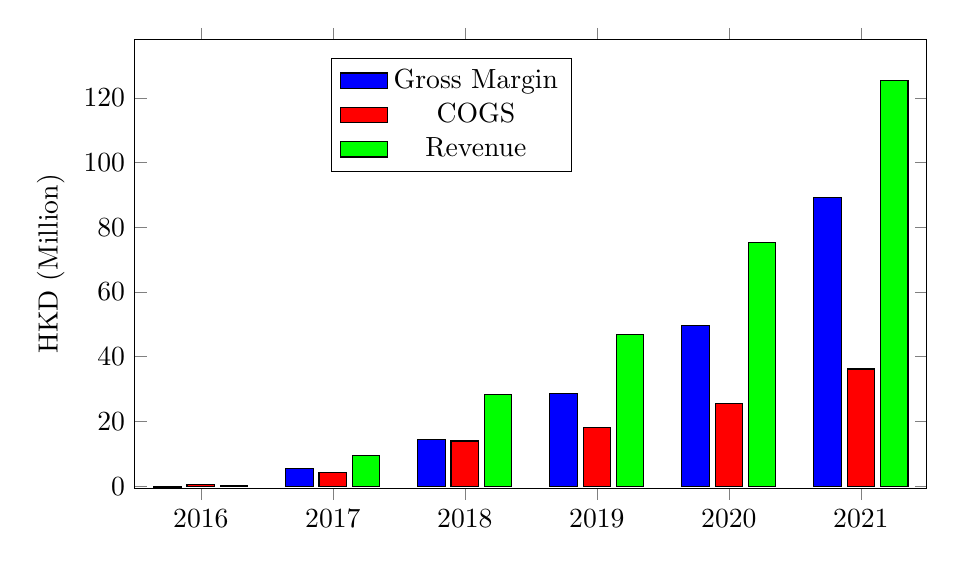
\begin{tikzpicture}
\begin{axis}[
width=0.96\linewidth,
height=0.60\linewidth,
%ybar stacked,
ybar,
area legend,
legend style={at={(0.4,0.96)}, anchor=north},
symbolic x coords={2016, 2017, 2018, 2019, 2020, 2021},
xtick=data,
ymin=-0.6,
ylabel=HKD (Million),
enlarge x limits=0.1
]
\addplot[ybar,fill=blue] coordinates {
    (2016, -0.400000) (2017, 5.36) (2018, 14.443) (2019, 28.688) (2020, 49.758) (2021, 89.177)
};
\addplot[ybar,fill=red] coordinates {
    (2016, 0.500000) (2017, 4.24) (2018, 13.957) (2019, 18.072) (2020, 25.506) (2021, 36.193)
};
\addplot[ybar,fill=green] coordinates {
    (2016, 0.100000) (2017, 9.6) (2018, 28.4) (2019, 46.760) (2020, 75.264) (2021, 125.3696)
};
\legend{Gross Margin, COGS, Revenue};
\end{axis}
\end{tikzpicture}
	\caption{Rough financial projections of Pear in 5 years.} \label{fig:financial-projections}
\end{figure}

\subsubsection{Exit Strategy and IRR}
Table~\ref{tb:exit-strategy-irr} shows the exit strategy and the corresponding return rate. 
\begin{table}[htbp]
	\centering
	\caption{Exit Strategy and IRR}\label{tb:exit-strategy-irr}
	\begin{tabular}[t]{lrrr}  
		\toprule
		Cases & Optimistic & Baseline & Pessimistic\\
		\midrule
		Exit Strategy & IPO & Buy Back & M\&A\\
		NPV (HKD) & 355,829,000 & 33,778,000 & 5,648,000\\
		IRR & $242\%$ & $93\%$ & $51\%$\\
		\bottomrule
	\end{tabular}
\end{table}

\subsubsection{Use of Investment}
Table~\ref{tb:use-of-investment} shows the use of investment which can be roughly divided into four parts.  
\begin{table}[htbp]
	\centering
	\caption{Use of Investment}\label{tb:use-of-investment}
	\begin{tabular}[t]{ccccc}  
		\toprule
		Total & Pilot \& Field testing & R \& D & Marketing & G \& A\\
		\midrule
		$6,000$ K & $1,500$ K & $3,800$ K & $500$ K & $200$ K\\
		\bottomrule
	\end{tabular}
\end{table}

In this recession \& capital winter, Pear will spend about two-thirds of its Series Pre-A round funding on R\&D, in order to build finely crafted products, competitive advantages and barriers to market entry. 
This long-term investment will generate unexpected results in ``winter to spring'', when there will be a lot of cheap resources ({\em e.g.} dying O2O companies' legacies) available to obtain.

\newpage
